\documentclass{report}
\usepackage[papersize={8.5in,11in}, margin=0.4in, bottom = 1.3in, headsep=.3in]{geometry}
\usepackage[utf8]{inputenc}
\usepackage{setspace}
\usepackage{amssymb}
\usepackage{amsmath}
\usepackage{physics}
\usepackage{fancyhdr}
\usepackage{ragged2e}
\usepackage[none]{hyphenat}%%%%
\usepackage[scr]{rsfso}
\usepackage{physics}
\usepackage{graphicx}
\usepackage{hyperref}
\usepackage{enumitem}
\usepackage{tikz}

\hypersetup{
    colorlinks=true, %set true if you want colored links
    linktoc=all,     %set to all if you want both sections and subsections linked
    linkcolor=blue,  %choose some color if you want links to stand out
}

\usetikzlibrary{positioning}

\addtolength{\topmargin}{.5in}

\pagestyle{fancy}
\fancyhf{}
\fancyhead[L]{The Cooper Union \\ESC251 - System Dynamics\\Prof. Luchtenburg}
\fancyhead[R]{Benjamin Aziel  \\Spring 2023\\}
\setlength{\headheight}{23pt}

\newcommand{\Laplace}{\mathscr{L}}
\newcommand{\UnitStep}{\mathscr{U}}
\newcommand{\Integer}{\mathbb{Z}}
\newcommand{\Natural}{\mathbb{N}}
\newcommand{\Volume}{{\ooalign{\hfil$V$\hfil\cr\kern0.08em--\hfil\cr}}}

\newcommand{\bicture}[1]{
\begin{center}
    {\includegraphics[height=4cm]{#1}}
\end{center}}

\begin{document}

\thispagestyle{empty}
\title{\textbf{System Dynamics}}
\date{Spring 2023}
\author{Benjamin Aziel\\ The Cooper Union}
\maketitle



\thispagestyle{empty}
\begin{onehalfspacing}
\tableofcontents

\begin{flushleft}
\chapter{Course Overview and Motivation}

\section*{Preface}

The course is called Systems Engineering in the course catalog, but Prof. Luchtenburg informally calls it System Dynamics. It's a more apt name for what the course actually covers; if you look up Systems Engineering you'll find a completely different subject.

\medskip

The course text is Ogata's \textit{System Dynamics}, which is a pretty lousy book, I'd recommend reading the first few chapters of Nise or FPE instead. I can provide PDFs if you can't find them yourselves. Read the syllabus, it's pretty in depth.

\medskip

Prof. Luchtenburg \textit{should} put his notes up in the MS Teams Class Notebook and record his lectures. Your mileage may vary if you don't bother coming to class.

\medskip

Most figures here are taken from Prof. Luchtenburg's Class Notebook. When I take figures from another source, I will mention it there. This document is a living document, which means I'll continue editing it as I see fit.

\medskip

I have this lousy habit of writing in the fourth person and cursing in my writing. Apologies in advance.

\section{Why Model?}

Good question.

\pagebreak

\chapter{The First Order}

\section*{Preface}

Let's start by throwing out some systems and testing familiarity with first-order systems and simplified models.
\begin{itemize}[noitemsep,topsep=0.5pt]
    \item Emptying a water tank
    \item Cooling of a lightbulb
    \item Discharge of an RC circuit
\end{itemize}

\section{Gradients Make Stuff Flow (Very Hand-Wavey Edition)}

\bicture{1_sys1}

A cylindrical tank is filled to a level \(h\), has a cross-sectional area of \(A\), and an outflow rate of \(Q_\text{out}\). The pressure outside the tank is \(P_{\infty}\). Can we derive a governing equation for this system? Well, we can try with a few physical principles.

\medskip

Let's start with a \textbf{conservation law}. We know there's a volume \(\Volume\) of water proportional to the value of \(h\). Or\dots

\vspace{-0.1in}
\[\Delta \Volume = A \Delta h\]

We'll take the time derivative of that equation to get some more familiar variables. (You might recognize the math here from related rates in Ma111.)

\vspace{-0.1in}
\[\frac{d}{dt} \qty[\Delta \Volume = A \Delta h] = -Q_\text{out}\]

That's not very useful yet. Let's leverage some prior circuits knowledge here...charge moves because of a \textbf{voltage difference} \(\Delta V\), and comparably, fluid moves because of a \textbf{pressure difference}. Ohm's law! We'll come back to that, but the main takeaway here is that the outflow \(Q_\text{out}\) is related to the difference between the pressure inside the tank \(P\) and the atmospheric pressure \(P_\infty\).

\medskip

That circuits analogy comes in handy really often, because it turns out Ohm's law translates directly into fluid flow. 

\vspace{-0.1in}
\[\Delta V = V - V_0 = IR\]
\[\Delta P = P-P_\infty = Q_\text{out} R\]

These are called \textbf{constitutive equations}, or relationships between physical quantities. (The flow is proportional to a level difference, or gradient.)

\medskip

We'll generalize a bit soon, but for now I understand if you don't get it. It's still very hand-wavey.

\medskip

Let's leverage some hydrostatics now. The tank is open to the atmosphere at the top, so we can actually derive an expression for \(P\), the pressure at the base of the tank. We'll also define \(\rho\), the density of the fluid, and \(C\), or capacitance, as \(\frac{A}{\rho g}\), because it ends up being useful in the circuit analogy.\footnote{You'll see this technique leveraged again in ME342.}

\vspace{-0.1in}
\[\Delta P = \rho g \Delta h = \rho g \frac{\Delta \Volume}{A} = \frac{1}{C} \Delta \Volume\]
\[C = \frac{A}{\rho g}\]

OK, I think we're all set. I've been pretty lax with the ``delta's", but it should still be readable. Let me know if things need clarification.

\vspace{-0.1in}
\[\dot{\Volume} = -Q_\text{out}\]
\[C \dot{\Delta P} = - \frac{\Delta P}{R}\]
\[\boxed{RC \dot{\Delta P} + {\Delta P} = 0}\]

This is a really nice differential equation. It looks like the equation for an RC circuit if you've seen those before, with the voltage differentials swapped out for pressure differentials.

\medskip

Let's move onto a second example: the cooling of a lightbulb. When we shut off power to the lightbulb, how can we measure its temperature as it cools to room temperature?

\bicture{1_sys2}

The bulb is initially very hot (with temperature \(T\)) compared to its environment (which has temperature \(T_\infty\)). Heat is flowing outwards at \(\dot{q}_\text{out}\).\footnote{I'm not a fan of the usual notation here, so I'm using \(\dot{q}\) for the flow of heat and \(q\) for heat.} This is seeming very familiar...a temperature difference is driving heat to leave through the resistance \(R\) of the bulb.

\medskip

Let's go through the steps again. What's being conserved here?\footnote{Someone said kinetic energy. What a statistical mechanics-esque answer.} Internal energy! (Or heat, since there's no work in this system.) It might be a bit early in the semester to have seen the capacitive relationship relating heat \(q\) and temperature \(T\) in ESC330, but here it is:

\vspace{-0.1in}
\[\Delta q = C \Delta T\]

Differentiate across the board\dots

\vspace{-0.1in}
\[\frac{d}{dt} \qty(C \Delta T) = C\dot{T} = -\dot{q}_\text{out}\]

And now we're just chugging through the motions. Next is another constitutive relationship (which looks shudderingly close to Ohm's law!):

\vspace{-0.1in}
\[\Delta T = T - T_\infty = \dot{q}_\text{out} R\]

Using this and the conservation equation, we construct:

\vspace{-0.1in}
\[\boxed{RC \dot{\Delta T} + \Delta T = 0}\]

Again. Familiar. Very familiar. Maybe there's some unifying theory in the background here.

\section{Solving that Damn Equation (and Time Constants)}

We'll generalize that equation to what we call its \textbf{canonical form} \(\tau \dot{y} + y = 0\), a first order differential equation. Let's throw in an initial condition \(y(0)=y_0\) just so we don't have any undetermined constants at the end.

\medskip

To solve this differential equation, we'll guess a solution \(y(t) = ce^{\alpha t}\), find its time derivative \(\dot{y}(t) = \alpha ce^{\alpha t} = \alpha y\), and plug in.

\vspace{-0.1in}
\[\tau \dot{y} + y = 0\]
\[\tau \alpha e^{\alpha t} + e^{\alpha t} = 0\]
\[(\tau \alpha + 1) \; e^{\alpha t} = 0\]
\[\alpha = -\frac{1}{\tau}\]
\[y(t) = ce^{-\frac{t}{\tau}} = y_0 \; e^{-\frac{t}{\tau}}\]

If you look at the graph below, it's just exponential decay from \((0, y_0)\). We call \(\tau\) the \textbf{time constant} of the system, and it's commonly used to describe how quickly an exponential decays or grows. Different systems have different time constants. (Notably, \(RC\) always has units of time). The smaller the time constant, the faster the decay. (Assume for the figure below that \(\tau_1 = 10\) and \(\tau_2 = 5\).)

\bicture{2_exp}

So what happens when we set \(t=\tau\)? Let's plug it in and find out.

\[y(\tau) = y_0 e^{-\frac{\tau}{\tau}} = y_0 e^{-1}\]

So the time constant is the time at which the system response has decayed to \(y_0 e^{-1}\), or approximately 37\% of its initial value. We can also reframe this definition as, ``the time constant is the time at which the system response has lost approximately 63\% of its initial value''. There is a different definition of the time constant for increasing systems that we will explore in the next section.

\section{The RC Circuit and Final Generalization}

Say we have an RC circuit with a full capacitor. 

\bicture{2_rc}

The outflow of charge from the capacitor is represented as a negative current:
\vspace{-0.1in}
\[\dot{q} = -I_\text{out}\]

Here's Ohm's law:
\vspace{-0.1in}
\[V = I_\text{out} R = \dot{q} R\]

Finally, we deal in the capacitive relationship (from Ph213):
\vspace{-0.1in}
\[q = C\Delta V\]

Chug everything together and we get:
\vspace{-0.1in}
\[C\dot{\Delta V} = -\frac{\Delta V}{R}\]
\[\boxed{RC \dot{\Delta V} + \Delta V = 0}\]

which is the same equation we've gotten before. (Notably, we don't have to have this equation in terms of the voltage difference; as you'll see in ESC221 this semester, there's a form of the equation in terms of current as well.)

\medskip

Final takeaways:
\begin{itemize}[noitemsep,topsep=0.5pt]
    \item Most first order systems we'll analyze in this class are the same mathematically!
    \item \textbf{Level differences make stuff flow.}
\end{itemize}

\medskip

``Stuff'' isn't the greatest word for something like this, (maybe quantity instead?) but that's the best we have. Stuff can be stored, like charge in a capacitor, or fluid in a tank, or heat in a reservoir. However, by generalizing these quantities, we can create widely applicable rules for modeling first order systems.

\[\text{Stuff} = \text{Capacitance} \times \text{Level Difference}\]
\[\text{Level Difference} = \text{Flow of Stuff} \times \text{Resistance}\]

Also conservation. That's a biggie.
\[\text{Rate of Change of Stuff} = \text{Inflow} - \text{Outflow}\]

We've only discussed scenarios where there isn't anything flowing in thus far. In these cases, to solve nonhomogeneous differential equations, we'll have to use more specialized methods from Ma240 instead of guessing and praying, like the Laplace transform or the method of undetermined coefficients (or as I affectionately call it, MUC).

\section{Let's Throw in an Input}

A more simple form of the governing equation for one of these first order systems is:

\vspace{-0.1in}
\[\tau \dot{y} + y = ku\]

when we have a constant input. Think of it as turning on a light switch at time \(t=0\). \(k\) is just a scale factor, and \(u(t)\) is the unit-step function, which is just \(0\) when \(t<0\) and \(1\) when \(t>0\).\footnote{We don't care about what happens at \(t=0\). Stop it.}

\vspace{-0.1in}
\[y(t) = ce^{-\frac{t}{\tau}} + k\]

For the initial condition \(y(0) = y_0\), the undetermined coefficient \(c=y_0 - k\). Here's our updated solution:

\vspace{-0.1in}
\[y(t) = y_0 e^{-\frac{t}{\tau}} + k(1-e^{-\frac{t}{\tau}})\]

When we graph this function for \(y_0 = 0\), we see that it gradually grows towards \(y=k\) as \(t\to\infty\). Now we can analyze exponential growth. You see this behavior everywhere, like when you change a thermostat setting and the temperature slowly creeps towards your choice. This is what we call a \textbf{step response}.

\bicture{2_step}

How could we find the time constant of this response? Let's take a look at what happens to \(y(t)\) at \(t=\tau\).

\vspace{-0.1in}
\[y(\tau) = y_0 e^{-\frac{\tau}{\tau}} + k(1-e^{-\frac{\tau}{\tau}})= y_0 e^{-1} + k(1-e^{-1})\]

When we set \(y_0 = 0\), this further simplifies to:

\vspace{-0.1in}
\[y(\tau) = k(1-e^{-1}) \approx 0.63 k\]

For this system, at \(t=\tau\), the system response will have accumulated 63\% of its steady state value.

\medskip

The step input is just one of the test inputs we usually use; we'll look at a few more as the course progresses (such as sinusoidal waves, delta functions, etc.).

\chapter{Our Second Order of Business}

\section*{Preface}

First order systems are honestly pretty boring. When we put in a step input, we just get a pure exponential. We won't be able to get more interesting behavior, like oscillation, because that's just mathematically impossible.\footnote{Prove it!}

\medskip

Second order systems, on the other hand, \textit{can} oscillate by themselves. Try to convince yourself of this mathematically just based on what oscillation is.

\bicture{2_unf}

Mass-spring systems are pretty good models of everything in the world (as long as you use enough mass-spring systems). They're really nice because having a good understanding of ONE mass-spring system provides us with the intuition for more complicated systems. 

\medskip

Say we have a mass-spring system where a mass \(m\) is attached to a wall with a spring \(k\) and a damper \(b\). Gravity isn't ``turned on'', so if you want to visualize the system, that mass is floating. The equation of motion for a positive displacement \(q\) is:\footnote{Prof. Luchtenburg went off on a tangent about Hooke being a genius for realizing that spring motion is linear near the origin here. That was pretty funny.}

\vspace{-0.1in}
\[m\ddot{q} = -kq - b\dot{q}\]

Or in its more familiar form:

\vspace{-0.1in}
\[m\ddot{q} + b\dot{q} + kq = 0\]

This is the famed mass-spring equation. Say we have an input - a force \(u\) acting on the mass in the positive direction. Now our equation of motion is:

\vspace{-0.1in}
\[m\ddot{q} + b\dot{q} + kq = u\]

This is a linear differential equation, so we'll solve this by plugging in an educated guess. Let's try \(q(t) = Ae^{st}\), because differentiating this function \(n\) times just multiplies it by \(s^n\).

\vspace{-0.1in}
\[ms^2 Ae^{st} + bs Ae^{st} + kAe^{st} = u\]
\[ms^2 + bs + k = u\]

First, we'll solve the homogeneous equation, or the case where \(u=0\).\footnote{If you're curious why we do this, you can read up on it in a linear algebra textbook. Think it's theorem 3.9 in Friedberg's Linear Algebra.}

\[ms^2 + bs + k = 0\]

This is known as the characteristic (or auxiliary) equation. We can now use algebra to solve for the roots of the equation, or by proxy, the solution of the differential equation.

\[s_{1, 2} = \frac{-b \pm \sqrt{b^2 - 4mk}}{2m}\]

These are also called the \textbf{poles} of the system, but we're getting ahead of ourselves. Let's simplify further.

\[s_{1, 2} = \frac{-b \pm \sqrt{b^2 - 4mk}}{2m} = -\frac{b}{2m} \pm \sqrt{\frac{b^2 - 4mk}{4m^2}} = -\frac{b}{2m} \pm \sqrt{\qty(\frac{b}{2m})^2 - \frac{k}{m}}\]

We define the \textbf{natural frequency} \(\omega_n = \sqrt{\frac{k}{m}}\) and the \textbf{damping ratio} \(\zeta = \frac{b}{2m\omega_n}\). Using these definitions, we can reorganize the mass-spring equation in terms of these variables.

\vspace{-0.1in}
\[m\ddot{q} + b\dot{q} + kq = 0 \qquad \to \qquad \ddot{q} + 2\zeta\omega_n \dot{q} + \omega_n^2 q = 0\]

And the poles of this equation are:

\[s_{1, 2} = -\zeta \omega_n \pm \omega_n \sqrt{\zeta^2 - 1}\]

I just realized this is my second time having this lecture today, so I'm just going to copy-paste my ME301 notes here.

\section{Intermezzo - Complex Analysis}

Complex analysis is the study of functions of a complex variable \(z\), where \(z\) has a real component \(a\) and an imaginary component \(b\). Complex numbers show up all the time in this course, whenever anything oscillates, really (like mass-spring systems and pendula).

\medskip

To take our first plunge into complex analysis, we need to define the \textbf{imaginary unit} \(i\).\footnote{You'll see people, especially electrical engineers, use \(j\) instead, because \(i\) is commonly used for current. We're better than them.} For now, let's define \(i\) as one of the two solutions to the quadratic equation \(x^2 = -1\). (The other is \(-i\), of course.) This is really special, because now we can describe the solutions of ALL polynomials\footnote{Regardless if its coefficients are real or complex!} as the sum of a real number \(a\) and another real number \(b\) multiplied by the imaginary unit \(i\).

\medskip

Let's conjure up a graphical representation of these numbers using Cartesian coordinates, where we define one axis as ``real'' and the other as ``imaginary''. We'll call this the complex plane. An arbitrary point \(z = a+ ib\) is plotted below.

\bicture{2_cpx}

We can also interpret these numbers in the context of polar coordinates, where \(\theta\) is the angle between the vector from the origin to \(z\) and the real axis, and \(r\) is the magnitude of the aforementioned vector. It's not difficult to translate between Cartesian coordinates and polar coordinates, but I'll dump the formulas here anyway.

\vspace{-0.1in}
\[a = r \cos{\theta} \qquad b = r \sin{\theta} \qquad r = \sqrt{a^2 + b^2} \qquad \theta = \arctan\qty({\frac{b}{a}})\]

It'd be criminal to not mention Euler's formula\footnote{You can prove this using the Taylor series representation of \(e^{x}\). You should do it, it's \textit{very} rewarding}, which posits that:

\vspace{-0.1in}
\[e^{i\theta} = \cos{\theta} + i \sin{\theta}\]

A lot of the nuance of complex numbers is best understood by analyzing this \textbf{complex exponential}, especially because:

\vspace{-0.1in}
\[z = a+ib = r\cos{\theta} + ir \sin{\theta} = r (\cos{\theta} + i \sin{\theta}) = re^{i\theta}\]

\section{Damping (You Guys are Going to See This Over and Over and Over)}

When \(\zeta = 0\) (or the system is \textbf{undamped}), we have the poles \(s_{1, 2} = \pm i\omega_n^2\). This implies that our solution is a linear combination of sines and cosines, endlessly oscillating, forever and ever. (That's kind of depressing to be honest.)
\medskip

``\textit{What next? Euler guy.}''

\vspace{-0.1in}
\begin{flushright}
    -Prof. Luchtenburg
\end{flushright}

\vspace{-0.1in}
\[x(t) = A_1 e^{i\omega_n t} + A_2 e^{- i \omega_n t} \; \footnote{Apparently \(A_1\) and \(A_2\) are complex conjugates. Don't quote me on that.} = A_1 (\cos(\omega_n t) + i \sin(\omega_n t)) + A_2 (\cos(\omega_n t) - i \sin(\omega_n t))\]
\vspace{-0.3in}
\[= (A_1 + A_2) \cos(\omega_n t) + i(A_1 - A_2) \sin(\omega_n t) = C_1 \cos(\omega_n t) + C_2 \sin(\omega_n t)\]

This reasoning carries over if we pick a damping ratio \(\zeta\) between 0 and 1 (or the system is \textbf{underdamped}). The poles are:

\vspace{-0.1in}
\[s_{1, 2} = -\zeta \omega_n \pm \sqrt{\omega_n^2 (\zeta^2 - 1)} = -\zeta \omega_n \pm i \omega_n \sqrt{1 - \zeta^2} = \sigma \pm i \omega_d\] 

We define the \textbf{damped frequency} \(\omega_d = \omega_n \sqrt{1-\zeta^2}\). (In practice, \(\omega_d \approx \omega_n\), because \(\zeta \ll 1\).) Additionally, we define \(\sigma = i\omega_n\) (for some reason). After substituting these new variables in, our solution becomes:

\vspace{-0.1in}
\[x(t) = A_1 e^{(-\sigma + i\omega_d) t} + A_2 e^{(-\sigma - i\omega_d) t} = e^{-\sigma t} (C_1 \cos(\omega_n t) + C_2 \sin(\omega_n t))\]

In the lattermost form, it's obvious that \(\sigma\) in fact \textit{does} have a use other than bookkeeping; it defines the exponential \textbf{envelope} by which the oscillation decays. An envelope is a function that outlines how a function grows/decays (it's the red dashed line in the figure below).

\bicture{5_env}

Notably, the time constant \(\tau\) of the envelope is equal to \(1/\sigma\). Thus, we can eyeball the value of \(\sigma\) based on how we'd find the time constant (the value \(63\%\) less than the \(y\)-intercept of the envelope).

\vspace{-0.1in}
\[x(t) = e^{-\sigma t} \sin(\omega_d t + \varphi)\]

Most mechanical systems tend to have a very low damping ratio (\(\zeta \simeq O(0.1)\)\footnote{Related rates of growth from Ma111, or big-O notation if you've taken ECE264.}), and as mentioned before, a good rule of thumb is that \(\omega_n = \omega_d\).

\medskip

When we apply some initial conditions (like \(q(0) = q_0\) and \(\dot{q}(0) = v_0\)), our solution becomes:

\vspace{-0.1in}
\[q(t) = e^{\sigma t} \qty(q_0 \cos(\omega_d t) + \frac{\sigma q_0 + v_0}{\omega_d} \sin(\omega_d t))\]

When \(\zeta = 1\), or the system is \textbf{critically damped}, the poles are:

\vspace{-0.1in}
\[s_{1, 2} = -\zeta \omega_n\]

We use a trick from differential equations to fake another linearly independent solution, just chuck on an extra \(t\).

\vspace{-0.1in}
\[q(t) = A_1 e^{-\zeta \omega_n t} + A_2 t e^{-\zeta \omega_n t}\]

This doesn't really happen in the real world, but it's nice to cover all our bases. How about when \(\zeta > 1\)? We call this case \textbf{overdamped}, because our poles are:

\vspace{-0.1in}
\[s_{1, 2} = -\zeta \omega_n \pm \omega_n \sqrt{\zeta^2 - 1}\]

Both poles are negative here! Our solution is:

\vspace{-0.1in}
\[q(t) = A_1 e^{s_1 t} + A_2 e^{s_2 t}\]

\section{Pole Plots}

I've been emphasizing poles a lot in the last few pages, but why? What's the importance of these seemingly arbitrary values? In fact, we can infer the dynamics of a system based on its poles.\footnote{This is the crux of a lot we do in ME351. If any of you remember what an eigenvalue is from Ma110, that'll come in handy in a bit.}

\medskip

To analyze poles, we use a graphical tool called a \textbf{pole plot}, the plot of the roots of the characteristic equation on the complex plane. Let's go down the list:

\begin{itemize}[noitemsep]
    \item When both poles are on the imaginary axis, the system is undamped.
    \item When both poles are off the real axis, the system oscillates. If they're to the left of the imaginary axis, it'll decay exponentially (underdamped), and if they're to the right of the imaginary axis, it'll grow exponentially.
    \item If both poles are on the real axis to the left of the imaginary axis, it's overdamped.
    \item Rule of thumb: if there is ANY pole to the right of the imaginary axis, the response blows up.
\end{itemize}

Here's a nice chart from FPE. Complex conjugates are omitted for simplicity.

\begin{center}
    {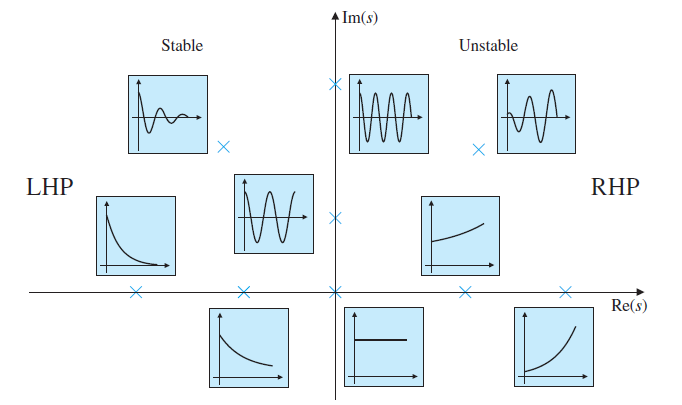
\includegraphics[height=8cm]{7_fpe}}
\end{center}



\section{Leveraging the Discriminant}

I'm going to stray off from Prof. Luchtenburg for a second because \textit{I} think this is useful.

\medskip

Suppose we want to identify the dampedness of a system based on the equation of motion rather than solving for \(\zeta\). We can do exactly this using the \textbf{discriminant} of the characteristic equation of the system. Let's take a look at the canonical mass-spring system with a damper once again.

\bicture{2_unf}

The equation of motion, assuming free motion, is:

\vspace{-0.1in}
\[m\ddot{q} + b \dot{q} + k q = 0\]

The characteristic equation is derived after plugging in \(q = e^{st}\).

\vspace{-0.1in}
\[ms^2 + bs + k = 0\]

As stated in the damping section, there are three forms of the general solution if there is damping present: both poles are real and distinct (the system is overdamped), both poles are real and equal (the system is critically damped), or both poles are complex conjugates (the system is underdamped). You may recall from Algebra that the discriminant of a polynomial can reveal some properties of the roots without actually computing them. The discriminant of a quadratic is defined as follows:

\vspace{-0.1in}
\[\text{Disc}(ax^2 + bx + c) = b^2-4ac\]

This is the argument of the square root in the quadratic formula. If this expression is positive, the solutions to the quadratic are real and distinct. If this expression is 0, then there is only one real solution to the quadratic. If this expression is negative, the solutions to the quadratic are complex. So physically, finding the discriminant of the characteristic equation of the mass-spring system will tell us how damped it is.

\vspace{-0.1in}
\[\text{Disc}(ms^2 + bs + k) = b^2-4mk\]

\vspace{-0.35in}

\begin{align*}
    b^2 - 4mk > 0 \quad &\to \quad \text{overdamped} \\
    b^2 - 4mk = 0 \quad &\to \quad \text{critically damped} \\
    b^2 - 4mk < 0 \quad &\to \quad \text{underdamped} \\
\end{align*}

\vspace{-0.35in}

And of course, if \(b=0\), then the system is undamped. 

\section{The Tank, Revisited (Inertia)}

Let's revisit the tank from our study of first order systems. However, we'll make one small change: the outflow pipe now has a defined length of \(L_p\). 

\bicture{6_inert}

Let's model the same way we've been doing thus far. First, a conservation law:

\vspace{-0.1in}
\[\dot{\Volume} = -Q\]

Next, ``Ohm's law'':

\vspace{-0.1in}
\[Q = \frac{\Delta P}{R} = \frac{P - P_\text{atm}}{R}\]

If we isolate a piece of the pipe (with length \(L_p\)) as shown below, we can demystify this system a bit.

\bicture{6_pipe}

Assuming the cross-sectional area of the pipe \(A_p\) is constant, the pressure force \(F_p = A_p \Delta P\) accelerates the fluid between the two ends of this pipe. Additionally, there is friction \(F_f = -QRA_p\) on the liquid caused by the resistance of the pipe. By leveraging Newton's second law of motion, we now have a relationship between the pressure difference \(\Delta P\) and the velocity of the water \(v\).

\vspace{-0.1in}
\[m \frac{dv}{dt} = F_p + F_f = A_p \Delta P - Q R A_p\]

The mass \(m\) of the fluid between the two ends of this pipe is equal to the product of the density of the fluid \(\rho\) and the volume between the two ends \(\Volume_p\). (Notably, the volume \(\Volume_p = A_p L_p\).)

\vspace{-0.1in}
\[\rho \, \Volume_p \, \frac{dv}{dt} = \rho A_p L_p \, \frac{dv}{dt} = A_p \Delta P - RQ A_p\]

Because the product of the cross-sectional area \(A_p\) and the fluid velocity \(v\) is equal to the volumetric flow rate \(Q\), we can rewrite this equation as follows:

\vspace{-0.1in}
\[\frac{\rho L_p}{A_p} \, \frac{dQ}{dt} = \Delta P - RQ\]

Ok, we can shed some light on what we're doing now. We define \textbf{inductance} (also referred to as \textbf{liquid-flow inertance} or \textbf{inertia}) as a term that describes the change in potential required for a unit rate of fluid flow. Inductance is the tendency of the fluid to move; it's created by the inertia of water flowing through the pipe. The mathematical definition of inductance is as follows:

\vspace{-0.1in}
\[L = \frac{\rho L_p}{A_p}\]

Note that this definition of inductance is only valid for flow systems, but analogous concepts occur in other fields (like inductors from circuit analysis)! Fluid components that have an inductance are analogous to these inductors, or mechanical components with inertia. 

\medskip

Let's wrap up this example. When we plug in the definition of \(L\) into our equation, a simple first order system rears its head.\footnote{The analog of this system in circuit analysis is called the RL circuit, which is often used as a passive filter.}

\vspace{-0.1in}
\[L \, \frac{dQ}{dt} + RQ = \Delta P\]

Let's throw it into canonical form so we can see its time constant.

\vspace{-0.1in}
\[\qty(\frac{L}{R}) \dot{Q} + Q = \frac{\Delta P}{R} \qquad \qquad \tau = \frac{L}{R}\]

To summarize, we've added a new tool to our arsenal: conservation of momentum (or Newton's second law). 

\vspace{-0.25in}
\begin{align*}
    \Delta P &= L \dot{Q} + RQ \\
    \dot{\Volume} &= -Q\\
    C \Delta P &= \Volume
\end{align*}
\vspace{-0.25in}

By combining these three equations, we can use tools from our studies of mass-spring systems to analyze\dots well \dots any second order system.

\vspace{-0.1in}
\[L \Delta \ddot{P} + R \Delta \dot{P} + \frac{1}{C} \Delta P = 0 \qquad \to \qquad \Delta \ddot{P} + \qty(\frac{R}{L}) \Delta \dot{P} + \qty(\frac{1}{LC}) \Delta P = 0\]
\[m \ddot{q} + b \dot{q} + k q = 0 \qquad \to \qquad \ddot{q} + \qty(\frac{b}{m}) \dot{q} + \qty(\frac{k}{m}) q = 0\]

We simply retrofit the definitions of the natural frequency \(\omega_n\) and damping ratio \(\zeta\) based on how we defined them for mass-spring systems to determine how the oscillations behave. Here's a quick example using the flow system analogy we've been using thus far:

\vspace{-0.1in}
\[\qquad \ddot{q} + 2\zeta\omega_n \dot{q} + \omega_n^2 q = 0 \quad \longleftrightarrow \quad  \Delta \ddot{P} + \qty(\frac{R}{L}) \Delta \dot{P} + \qty(\frac{1}{LC}) \Delta P = 0\]

\vspace{-0.25in}
\begin{align*}
    2 \zeta \omega_n = \frac{R}{L} \qquad &\longrightarrow \qquad \zeta = \frac{R}{2L \omega_n} = \frac{R\sqrt{LC}}{2L} = \frac{R}{2} \sqrt{\frac{C}{L}}\\
    \omega_n^2 = \frac{1}{LC} \qquad &\longrightarrow \qquad \omega_n = \frac{1}{\sqrt{LC}} = \frac{\sqrt{LC}}{LC}
\end{align*}

\pagebreak

\chapter{Cool Math Games}

\section*{Preface}

This chapter's going to be a smorgasbord of mathematical concepts I think are foundational to understanding this course from a theoretical perspective. A decent chunk of it will be review from Ma240, but it doesn't hurt to take a second look at these things (they keep coming back over and over).

\medskip

What I'll try to do, instead of rehashing what you got out of Ma240, is reframe these concepts in a way that's more applicable to this course (and ME351).

\section{Linearity and Time Invariance}

Most of the mathematical models we end up creating are horribly limited, because the world is inherently unpredictable. In this class, we try our best to make do with \textbf{linear time invariant (LTI)} systems. 

\medskip

An LTI system is a mathematical model often used in control theory to describe the behavior of physical systems. It is characterized by two properties: linearity and time invariance. I'll describe these separately in the context of differential equations. A differential equation of the form:

\vspace{-0.1in}
\[a_n y^{(n)} (t) + a_{n-1} y^{(n-1)} + \dots + a_1 \dot{y}(t) + a_0 y(t) = f(t)\]

where \(y^{(i)}\) is the \(i\)th derivative of \(y(t)\), is called \textbf{linear}. (The relationship between \(y(t)\) and \(t\) is a linear mapping.) If \({a_i}_0^n\), also called coefficients, are constants, the equation is also characterized as a \textbf{constant coefficient} differential equation. Physically, constant coefficients imply that the system behavior does not depend on time. 

\medskip

We can establish an equivalence between linear constant coefficient equations and linear time invariant systems. Time invariance is the principle that if we chug an input \(t_0\) into a system that outputs \(y(t_0)\), the input \(t_0 + t_1\) will result in an output of \(y(t_0 + t_1)\). 


Let's take a look at a few examples to make this more clear:

\vspace{-0.1in}
\[\dot{y} + \sin(t) y = 0\]

This system is not LTI, because the coefficient of \(y\) is not constant. (More explicitly, it's a function of \(t\), so as \(t \to \infty\), the behavior is affected.)

\vspace{-0.1in}
\[2 \dot{y} + 3 y = 0\]

This system \textit{is} LTI, because the coefficients of each derivative of \(y\) are constant.

\vspace{-0.1in}
\[\dot{y} + \ln(y) = 0\]

This system isn't even linear, for obvious reasons.

\medskip

I'm skipping a lot of nuance here, and Prof. Mintchev would chop my head off if I showed him these lousy definitions. Nevertheless, we're engineers and not mathematicians.\footnote{In all seriousness, taking Ma326 was really cool, and I highly recommend it if you're interested in having the mathematical foundation necessary to learn more about dynamical systems.}

\section{Yay! More Linear Differential Equation Theory}

We've brushed upon how to solve first and second order linear differential equations that are \textbf{homogeneous}, or when the input \(f(t) = 0\).\footnote{If you don't remember, it's by plugging in a guess solution \(e^{st}\).} The generalization to \(n\)th order linear differential equations is pretty self explanatory.

\medskip

Here're a few tenets that we should keep in mind.

\begin{itemize}[noitemsep,topsep=0.5pt]
    \item yeah this is a tomorrow problem
\end{itemize}

\section{MUC (and Added Complexity)}

muckkkkkkkkkkkkkkkkkkkkkkkkkkkkk

\section{The State-Space Approach}

When we begin to analyze more complicated systems, it becomes less and less feasible to solve them analytically. As a result, we resort to setting up a system of differential equations rather than concatenating them into one as we've done in past chapters.

\medskip

The state-space representation of a system describes the system's behavior over time in terms of a set of variables called \textbf{states}.\footnote{The state space can be described as a Euclidean space where each state corresponds with an axis.} The state variables represent the current conditions of the system, and their evolution over time is described by a set of first order differential equations called \textbf{state equations}.

\medskip

The state-space representation is a very powerful tool for modeling and analyzing physical systems, providing valuable insights into their behavior and enabling the development of control algorithms covered in ME351.

\medskip

An important thing to note is that the state-space representation of a system is not unique. In fact, an infinite number of representations exist for a physical system.

\medskip

When constructing a representation, it is advantageous to represent the system in a minimal form without meaningless states. Usually, the number of necessary states to properly describe a physical system is equal to the order of the differential equation.

\medskip

In the most general case, a state-state representation can be represented as the following:

\begin{equation*}
    \left\{ \begin{array}{ll}
        \underbar{\(\dot{x}\)} = \underbar{\(f\)}(\underbar{\(x\)}, \underbar{\(u\)}) \\
        \underbar{\(y\)} = \underbar{\(h\)}(\underbar{\(x\)}, \underbar{\(u\)})
    \end{array} \right.
\end{equation*}

Ah, by the way, underlined quantities are vectorial.

\medskip

This might be a bit daunting at first, but it's just a lot of fancy notation for a concept that's pretty simple. \(\underbar{\(x\)}\) is the state, \(\underbar{\(u\)}\) is an input, and \(\underbar{\(y\)}\) is an output. Let's drive this concept home with an example.

\medskip

Say we have a simple pendulum with length \(L\) and a point mass \(m\) at its end, as pictured below:

\bicture{8_pend}

For this problem, the mass of the rod (and any potential friction in the hinge) is ignored. The equation of motion of the pendulum can be derived by summing moments about the point of contact between the pendulum and the fixed surface.\footnote{Alternatively, you could sum forces in the parallel and perpendicular directions of motion to yield an equivalent result.} Let's call that point of contact \(O\) for future bookkeeping purposes.

\vspace{-0.1in}
\[\sum{M_O} = J_O \ddot{\theta}\]

The moment arm for the weight \(mg\) is the horizontal displacement \(L \sin(\theta)\), and \(J_O = mL^2\) is the mass moment of inertia of the point mass \(m\) about point \(O\). Let's crunch some numbers.

\vspace{-0.1in}
\[-mgL \sin(\theta) = mL^2 \ddot{\theta}\]
\[mL^2 \ddot{\theta} + mgL \sin(\theta) = 0\]
\[\ddot{\theta} + \frac{g}{L} \sin(\theta) = 0\]

Now let's try putting this in state-space form. We define states \(\theta\) (angle) and \(\omega = \dot{\theta}\) (angular velocity), and start constructing our state equations.

\vspace{-0.1in}
\[\underbar{\(x\)} = \begin{bmatrix}
    \theta \\
    \omega  \end{bmatrix} \qquad \qquad \underbar{\(\dot{x}\)} = \begin{bmatrix}
        \dot{\theta} \\
        \dot{\omega}  \end{bmatrix}\]
\[\underbar{\(\dot{x}\)} = \underbar{\(f\)} (\underbar{\(x\)}, \underbar{\(u\)})\]
\vspace{-0.1in}
\[\dot{\underbar{\(x\)}} = \begin{bmatrix}
    \dot{\theta} \\
    \dot{\omega}  \end{bmatrix} = \begin{bmatrix}
    \omega \\
    -\frac{g}{L} \sin(\theta) 
\end{bmatrix}\]

We've turned a second order differential equation into two first order differential equations. Let's move onto the second part of the representation: defining the output \(y\). We're interested in the states' behavior over time, so our output is...just the state vector \underbar{\(x\)}.

\[\underbar{\(y\)} = \underbar{\(h\)}(\underbar{\(x\)}, \underbar{\(u\)}) = \underbar{\(x\)} = \begin{bmatrix}
    \theta \\
    \omega  \end{bmatrix}\]

These two components make up the state-space representation of this pendulum system. Putting it in this form makes it easier to numerically solve using tools like Python or MATLAB.

\medskip

A nonlinear solution can be unappealing, though perfectly valid. By using the small-angle approximation \(\sin(\theta) \sim \theta\), we can refine this representation further.

\[\ddot{\theta} + \frac{g}{L} \sin(\theta) \sim \ddot{\theta} + \frac{g}{L} \theta = 0\]

Our system is now an LTI system. Linearity is very nice, because we can use matrix multiplication to make this representation pretty.

\vspace{-0.1in}
\[\dot{\underbar{\(x\)}} = \begin{bmatrix}
    \dot{\theta} \\
    \dot{\omega}  \end{bmatrix} = \begin{bmatrix}
    \omega \\
    -\frac{g}{L} \theta
\end{bmatrix} = \begin{bmatrix}
    0 & 1\\
    -\frac{g}{L} & 0
\end{bmatrix} \begin{bmatrix}
    \theta \\
    \omega  \end{bmatrix}\]
\[\underbar{\(y\)} = \begin{bmatrix}
    \theta \\
    \omega  \end{bmatrix} = \begin{bmatrix}
        1 & 0\\
        0 & 1
    \end{bmatrix} \begin{bmatrix}
        \theta \\
        \omega  \end{bmatrix}\]

        
Let's say the pendulum had an input \(u\), and the new equation of motion was:

\vspace{-0.1in}
\[\ddot{\theta} + \frac{g}{L} \theta = \frac{u}{mL}\]





\section{The Laplace Transform}

ignore this i just wanna remember this when i start writing this section

The Laplace transform of the LTI derivative operator \(\dot{x}\) is just \(sX(s)\).



For a system with several variables, 

For an \(n\)th order system, we write \(n\) first-order differential equations in terms of the states.

do the pendulum example here, including the derivation of the EoM

maybe a footnote about how you can approximate \(g\) with a quick pendulum test

\end{flushleft}
\end{onehalfspacing}
\end{document}
